A continuación se presenta un análisis comparativo de los tres métodos implementados.
Cabe mencionar que, dado que la experimentación requería que ambas imágenes (original y modificada) tengan el mismo tamaño para poder realizar un análisis cuantitativo de los algoritmos mediante las medidas de comparación que se mencionaron en la introducción, decidimos achicar la imagen original mediante un programa de edición de imágenes para luego agrandarla mediante nuestros métodos y poder comparar los resultados obtenidos con la imagen original.

\subsection{Ventana óptima para método de Splines}
Nuestro primer análisis se encargará de encontrar un valor óptimo para la cantidad de las ventanas utilizadas en el método de splines.
Para dicho fin, elegimos correr varias instancias del método con valores de $K$ crecientes para distintos valores de ventana (4, 8, y 16 para poder comparar los resultados). Se presentan entonces los resultados obtenidos. Vale la pena destacar que no se muestra información respecto al PSNR debido a que presentaba exactamente el mismo comportamiento y no ofrecia informacion extra alguna.
\\
Como habiamos presupuesto en la introducción, agrandar el tamaño de la ventana solo hace que se tengan en cuenta valores para el punto que se quiere calcular que no depende directamente de este. 

\begin{center}
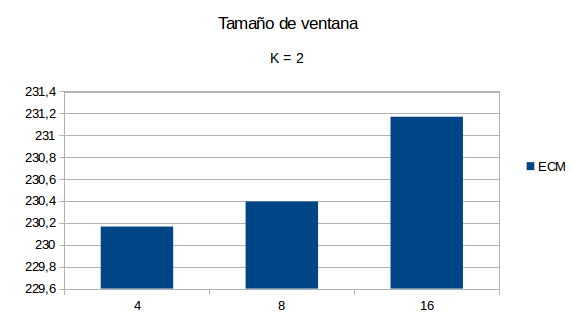
\includegraphics[scale=0.50]{imagenes/VK2.png}
\end{center}

Como puede verse a continuación, agrandar el tamaño de la ventana deja de presentar benificio alguno para valores mas altos de $K$ porque los resultados se veulven constantes:

\begin{center}
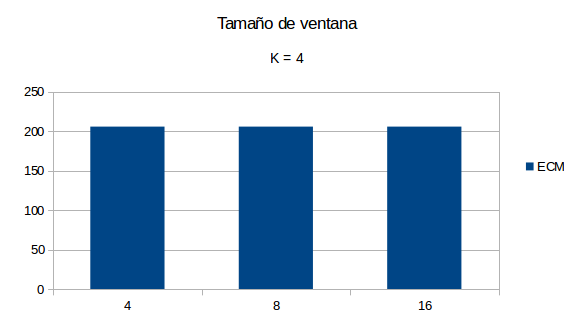
\includegraphics[scale=0.50]{imagenes/VK4.png}
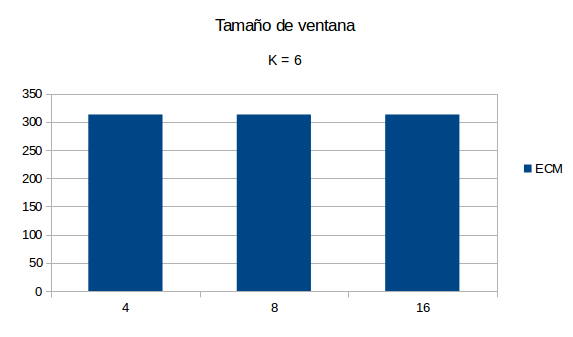
\includegraphics[scale=0.50]{imagenes/VK6.png}
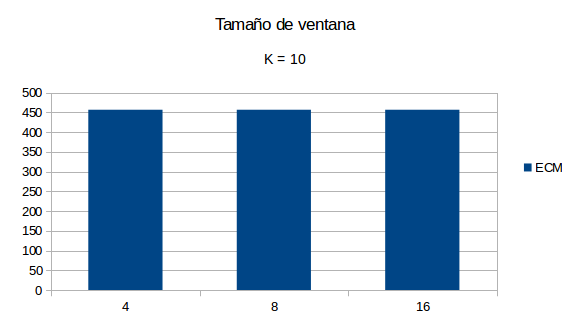
\includegraphics[scale=0.50]{imagenes/VK10.png}
\end{center}

A partir de este punto, el algoritmo de splines utiliza una ventana de tamaño cuatro, dado que es la que presenta mejores resultados.
De todos formas, no es cierto que siempre sea preferible una ventana más chica a una que incluya mas puntos, porque en problemas donde se quieren calcular por ejemplo trayectorias, es deseable considerar mas puntos para tener mas información.

\subsection{Análisis de los metodos}

Empleamos un análisis incremental respecto al valor de los pixeles intermedios introducidos (el valor de $k$) para poder analizar los distintos métodos de forma escalonada y presentar conclusiones mucho más claras. Dado que nuestros algoritmos solo funcionan cuando los valores de las imágenes son divisibles por $k$, no deben asumirse una correlación entre los distintos valores de este debido a que las imágenes a analizar no siempre pudieron ser las mismas.

\subsubsection{K = 2}
Nuestro primer análisis se concentra en el valor mínimo de $k$ para el cual esperabamos que el comportamiento de los tres métodos se mantenga bastante estable. Nuestra intuición proviene de la idea de que todos ellos ofrecian una perdida en la calidad de la imagen bastanta pequeña en relación al zoom pedido.
Como podemos apreciar en los gráficos a continuación, nuestra intuición se corresponde con los valores de $PSNR$, donde los tres métodos se comportan relativamente iguales, sin embargo, nos sorprende ver que para el error cuadrático medio (y para $PSNR$ también, pero en menor medida) la técnica de interpolación Bilineal obtuvo resultados muy destacables (de hecho, casi constantes), incluso frente a la técnica de Splines que esperabamos siempre tenga un mejor rendimiento. La conclusión respecto de este fenómeno se explica al final del artículo.

\begin{center}
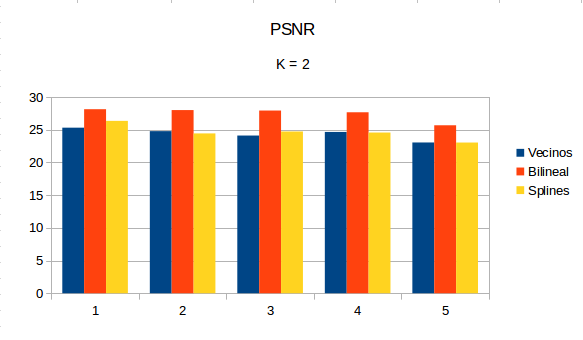
\includegraphics[scale=0.50]{imagenes/K2PSNR.png}
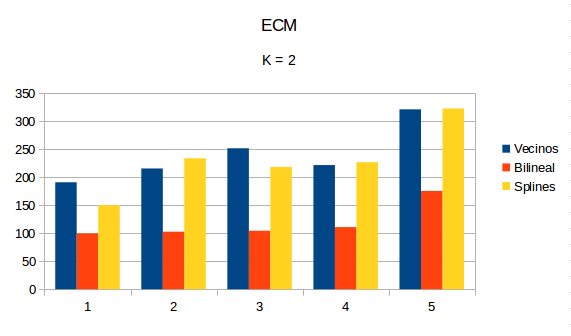
\includegraphics[scale=0.50]{imagenes/K2ECM.png}
\end{center}

\subsubsection{K = 4}
Para este segundo caso es cierto que, como esperabamos, el error cuadrático medio del método de los vecinos se dispara rápidamente mientras que los de interpolación bilineal y splines se mantienen prácticamente iguales. Lo mismo sucede para los valores de PSNR, siendo los del método de vecinos los únicos que disminuyen con una diferencia de casi 5 puntos.

\begin{center}
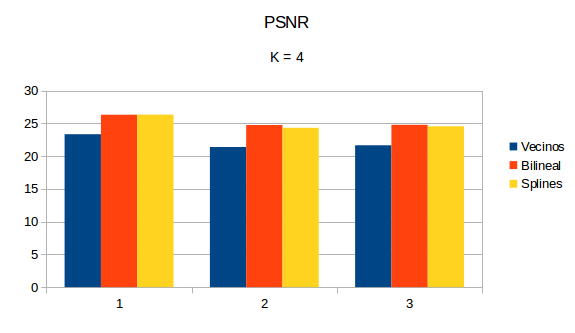
\includegraphics[scale=0.50]{imagenes/K4PSNR.png}
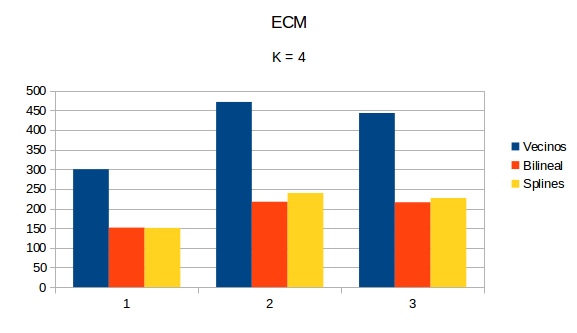
\includegraphics[scale=0.50]{imagenes/K4ECM.png}
\end{center}

\subsubsection{K = 6}
Entrando en valores de $k$ mucho más elevados, nuestro análisis empezó a dejar de coincidir con lo que creiamos en un primer momento serían los resultados finales, debido a que el método de Splines no logró sacar una diferencia notoria frente al de interpolación Bilineal, sino que incluso ambos métodos se mantuvieron prácticamente constantes.  Al momento de obtener los resultados nos llamaron poderosamente la atención los valores de ECM obtenidos para las tres primeras imágenes, pero luego de hacer un análisis en conjunto de estas, llegamos a la conclusión de que la suba desmesurada en estos valores se debe a la elevada variabilidad de los contrastes en la escena (el interior de un hogar muy decorado, la foto aérea de un barrio, etc). 

\begin{center}
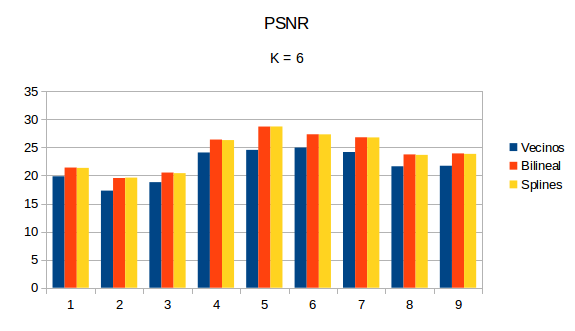
\includegraphics[scale=0.50]{imagenes/K6PSNR.png}
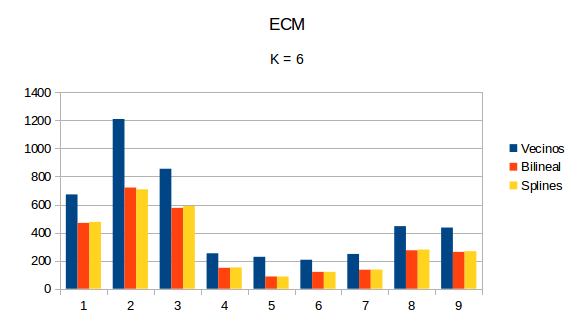
\includegraphics[scale=0.50]{imagenes/K6ECM.png}
\end{center}

\subsubsection{K = 10}
Por último, para valores que ya se consideran altos de $k$ el método de interpolación Bilineal todavía sigue desempeñandose igual o incluso a veces levemente mejor que el de Splines. Esto no solo contradice nuestra intuición, sino que debido a la performance de ambos, estos resultados colocan al método de interpolación como el más apto en relación benenficio/tiempo, muy por encima del de Splines (ambos ya muy por encima del método de vecinos a esta altura).

\begin{center}
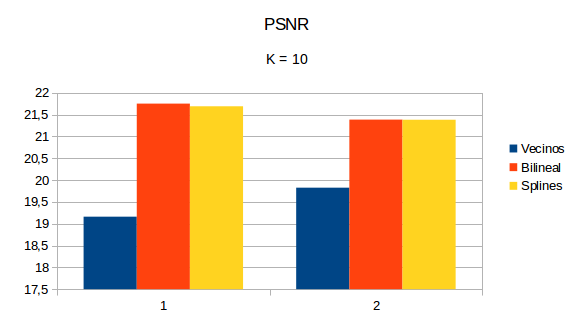
\includegraphics[scale=0.50]{imagenes/K10PSNR.png}
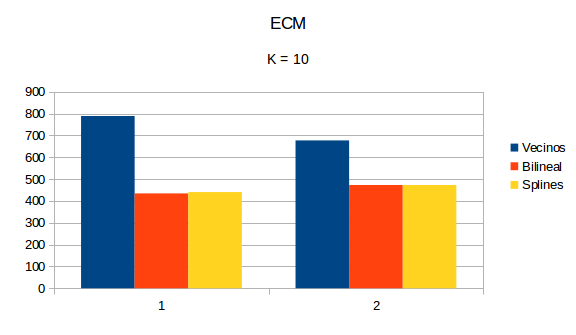
\includegraphics[scale=0.50]{imagenes/K10ECM.png}
\end{center}

\subsection{Análisis de tiempos}
El análisis de tiempo, a diferencia del de los métodos, no ofreció ninguna respuesta que no hayamos podido intuir durante la codificación de los algoritmos. Es claro que a medida que el método se perfecciona en la búsqueda de resultados más suaves, también aumenta el tiempo necesario de cálculo.

\begin{center}
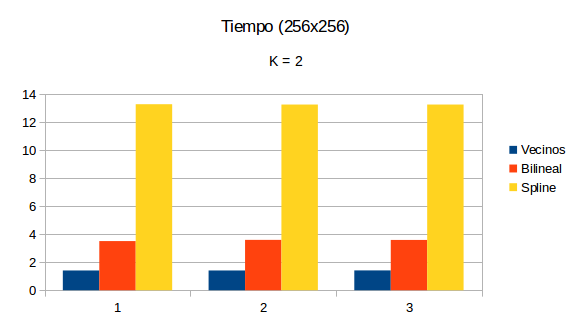
\includegraphics[scale=0.50]{imagenes/K2T1.png}
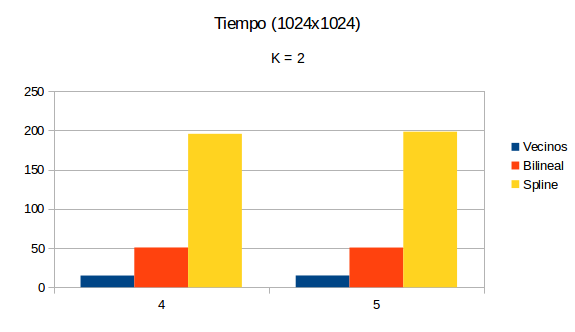
\includegraphics[scale=0.50]{imagenes/K2T2.png}
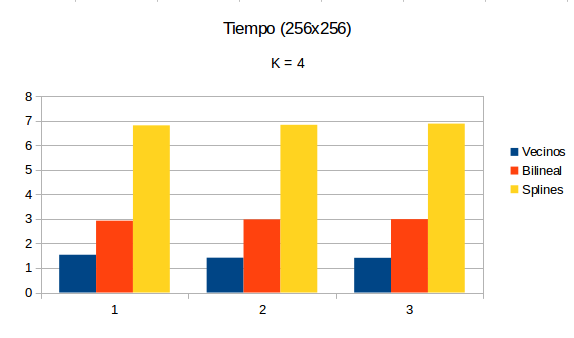
\includegraphics[scale=0.50]{imagenes/K4T.png}
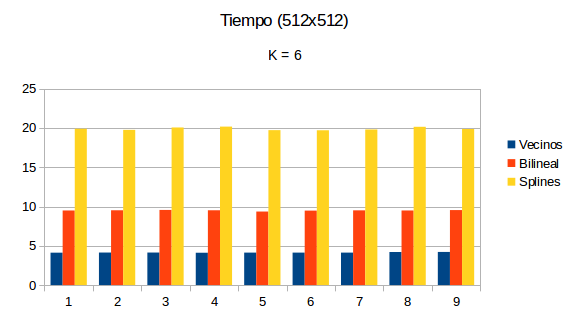
\includegraphics[scale=0.50]{imagenes/K6T.png}
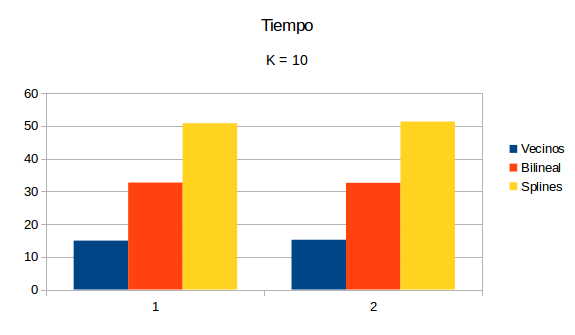
\includegraphics[scale=0.50]{imagenes/K10T.png}
\end{center}

\subsection{Analisis De Los metodos Para Imagenes Con Simbolos Alfanumericos}
En esta sección analizaremos los tres algoritmos sobre imagenes con simbolos alfanumericos. Para ellos usamos la imagen mostrada mas abajo para la cual aplicaremos los tres metodos con diferentes ks.

\begin{figure}[H]
\centering
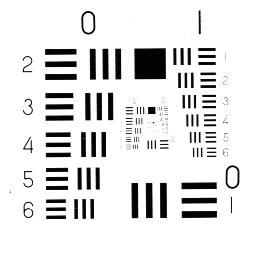
\includegraphics[scale=0.50]{fotos/alfanum/orig.png}
\end{figure}

Primero realizamos las pruebas con el valor minimo de $k$ ($k=1$), obteniendo los siguientes resultados:



\begin{figure}[H]
    \centering
    \subfloat[Metodo 1]{{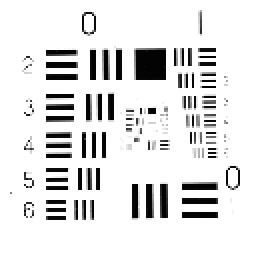
\includegraphics[width=5cm]{fotos/alfanum/k1_1.jpg} }}%
    \qquad
    \subfloat[Metodo 2]{{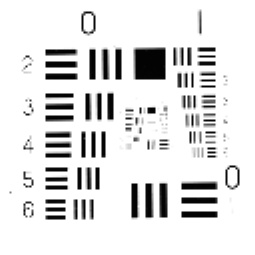
\includegraphics[width=5cm]{fotos/alfanum/k1_2.jpg} }}%
    \qquad
    \subfloat[Metodo 3]{{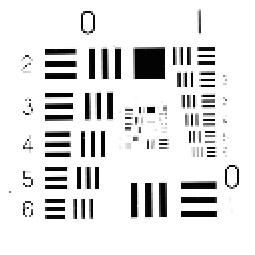
\includegraphics[width=5cm]{fotos/alfanum/k1_3.jpg} }}%
    \caption{Comparacón de metodos para $k = 1$}%
    \label{fig:example}%
\end{figure}

Como podemos ver, las tres imagenes introducen artifacts (errores visuales) que todavia no desmejoran la imagen a un nivel en el que sea imposible su comprension, por lo menos en los digitos mas externos (distinto para los numeros internos de la imagen que, debido a su tamaño inicial, ya son casi inperceptibles con este $k$ minimo). Notese como el metodo 2, como consecuencia de la nivelacion entre los valores de alto contraste del dibujo y su fondo blanco, empieza a introducir una leve 'niebla gris' alrededor de las imagenes. La misma sutiacion se plantea en el metodo tres, pero con la diferencia de que el difuminado introducido es mucho menos visible.

\\
Observemos los resultados para un $k$ un poco mas elevado ($k=2$):

\begin{figure}[H]
    \centering
    \subfloat[Metodo 1]{{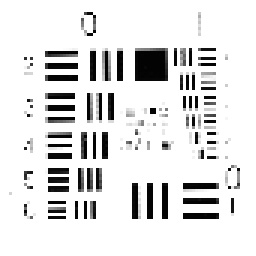
\includegraphics[width=5cm]{fotos/alfanum/k2_1.jpg} }}%
    \qquad
    \subfloat[Metodo 2]{{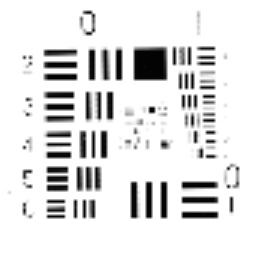
\includegraphics[width=5cm]{fotos/alfanum/k2_2.jpg} }}%
    \qquad
    \subfloat[Metodo 3]{{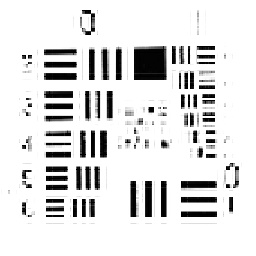
\includegraphics[width=5cm]{fotos/alfanum/k2_3.jpg} }}%
    \caption{Comparacón de metodos para $k = 2$}%
    \label{fig:example}%
\end{figure}

En esta ocacion, el comportamiento sigue los lineamientos generales del caso anterior, con la salvedad de que ninguna de las tres imagenes ya es comprensible. Vemos como la 'niebla' comentada en el caso anterior avanzo rapido en el metodo dos, para casi difuminar la imagen por completo. En el caso del metodo de splines (el tercero)se puede empezar a ver un pequeño sombreado alrededor de los bordes de los elementos en la imagen, pero a diferencia del metodo dos, esta solo se extiende a las cercanias y no avanza por toda la imagen.

\\
Por ultimo, presentamos los resultados para $k=4$:

\begin{figure}[H]
    \centering
    \subfloat[Metodo 1]{{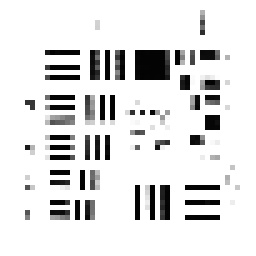
\includegraphics[width=5cm]{fotos/alfanum/k5_1.jpg} }}%
    \qquad
    \subfloat[Metodo 2]{{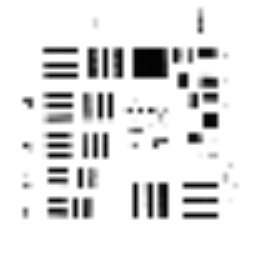
\includegraphics[width=5cm]{fotos/alfanum/k5_2.jpg} }}%
    \qquad
    \subfloat[Metodo 3]{{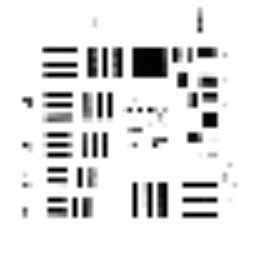
\includegraphics[width=5cm]{fotos/alfanum/k5_3.jpg} }}%
    \caption{Comparacón de metodos para $k = 4$}%
    \label{fig:example}%
\end{figure}

Como era de esperarse las tres imagenes resultantes ya perdieron comprension en su totalidad. Ademas, el segundo y tercer metodo, presentan una alta cantidad de ruido por el difuminado producido respecto de la imagen original.
Queda entonces a la vista una caracteristica que no estabamos considerando hasta entonces en nuestro analisis. El metodo de los vecinos puede llegar a ofrecer resultados favorables si se cumplen algunas caracteristicas deseables (nuestra intuición preveia que este metodo seria superado por los anteriores en cualquier situacion) como en este caso. El alto contraste entre las imagenes, hace que en los metodos que introducen cierta correlación o suavizado entre pixeles se genere un sombreado que hace mas borrosas las imagenes. En contra de nuestros pronosticos, el metodo de los vecinos podria ser un excelente candidato en estos casos.


\subsection{Analisis De Los metodos Para Paisajes}

En esta sección analizamos como se comportan los metodos para fotos de paisajes. Tomamos la siguiente foto:

\begin{figure}[H]
\centering
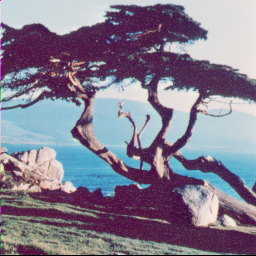
\includegraphics[scale=0.50]{fotos/paisaje/orig.png}
\end{figure}

Primero lo hacemos para $k=1$, se obtiene esto:

\begin{figure}[H]
    \centering
    \subfloat[Metodo 1]{{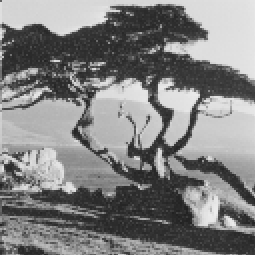
\includegraphics[width=5cm]{fotos/paisaje/k1_1.png} }}%
    \qquad
    \subfloat[Metodo 2]{{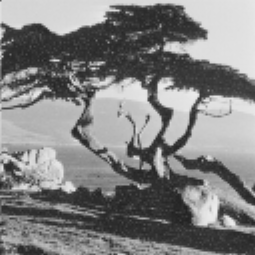
\includegraphics[width=5cm]{fotos/paisaje/k1_2.png} }}%
    \qquad
    \subfloat[Metodo 3]{{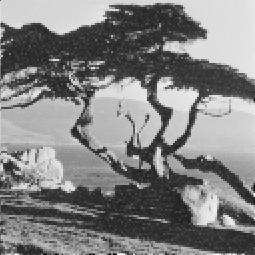
\includegraphics[width=5cm]{fotos/paisaje/k1_3.png} }}%
    \caption{Comparacón de metodos para $k = 1$}%
    \label{fig:example}%
\end{figure}

Los artifact (Errores visuales) que vemos aquí son, bla bla bla (COMPLETAR!). Ademas con el metodo $1$ nos dio un error cuadratico medio de $315.723$ y un psnr $23.1377$. Para el segundo metodo un error cuadratico medio de $115.114$ y un psnr $27.5195$ para el tercero $329.634$ y $22.9505$
\\
Ahora lo hacemos para $k=2$, se obtiene esto:

\begin{figure}[H]
    \centering
    \subfloat[Metodo 1]{{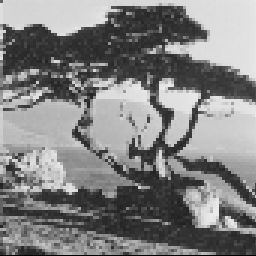
\includegraphics[width=5cm]{fotos/paisaje/k2_1.png} }}%
    \qquad
    \subfloat[Metodo 2]{{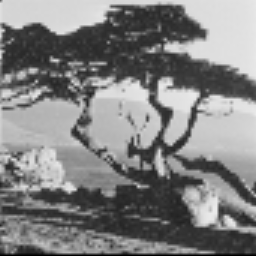
\includegraphics[width=5cm]{fotos/paisaje/k2_2.png} }}%
    \qquad
    \subfloat[Metodo 3]{{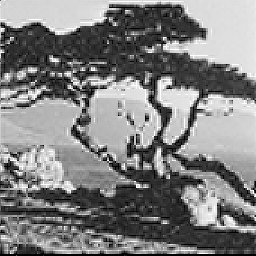
\includegraphics[width=5cm]{fotos/paisaje/k2_3.png} }}%
    \caption{Comparacón de metodos para $k = 2$}%
    \label{fig:example}%
\end{figure}

Los artifact que vemos aquí son, bla bla bla (COMPLETAR!)
%metodo 1
%ECM = 724.517 
%PSNR = 19.5303

%metodo 2
%ECM = 293.755
%PSNR = 23.4509

%metodo 3
%ECM = 938.898 
%PSNR = 18.4046
\\
Ahora lo hacemos para $k=3$, se obtiene esto:
\begin{figure}[H]
    \centering
    \subfloat[Metodo 1]{{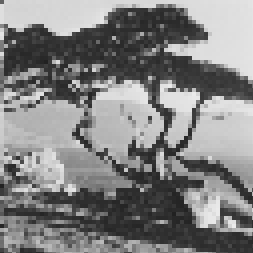
\includegraphics[width=5cm]{fotos/paisaje/k3_1.png} }}%
    \qquad
    \subfloat[Metodo 2]{{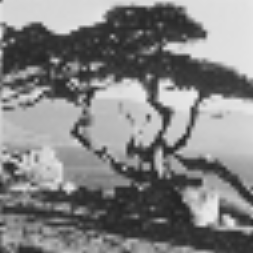
\includegraphics[width=5cm]{fotos/paisaje/k3_2.png} }}%
    \qquad
    \subfloat[Metodo 3]{{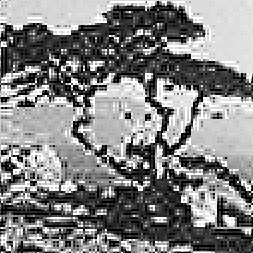
\includegraphics[width=5cm]{fotos/paisaje/k3_3.png} }}%
    \caption{Comparacón de metodos para $k = 3$}%
    \label{fig:example}%
\end{figure}

Obtenemos....
%metodo 1
%ECM = 1099.83 
%PSNR = 17.7175

%metodo 2
%ECM = 400.854 
%PSNR = 22.1009

%metodo 3
%ECM = 2992.94 
%PSNR = 13.3698

\subsection{Analisis De Los metodos para rostros}

En esta sección analizamos como se comportan los metodos para fotos de rostros. Tomamos la siguiente foto:

\begin{figure}[H]
\centering
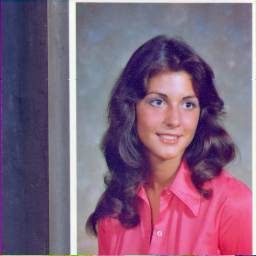
\includegraphics[scale=0.50]{fotos/rostro/orig.png}
\end{figure}

Primero lo hacemos para $k=1$, se obtiene esto:

\begin{figure}[H]
    \centering
    \subfloat[Metodo 1]{{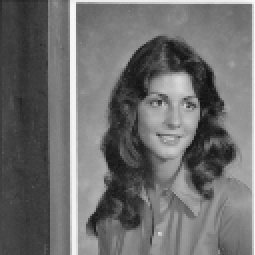
\includegraphics[width=5cm]{fotos/rostro/k1_1.png} }}%
    \qquad
    \subfloat[Metodo 2]{{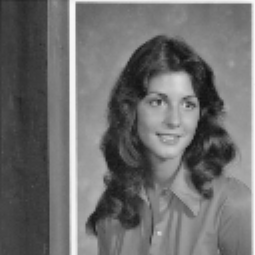
\includegraphics[width=5cm]{fotos/rostro/k1_2.png} }}%
    \qquad
    \subfloat[Metodo 3]{{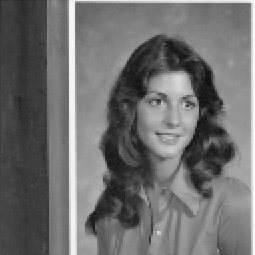
\includegraphics[width=5cm]{fotos/rostro/k1_3.png} }}%
    \caption{Comparacón de metodos para $k = 1$}%
    \label{fig:example}%
\end{figure}

Los artifact (Errores visuales) que vemos aquí son, bla bla bla (COMPLETAR!)
%metodo 1
%ECM        PSNR
%95.6087    28.3258
%metodo 2
%32.6121    32.997
%metodo 3
%104.209    27.9518
\\
Ahora lo hacemos para $k=2$, se obtiene esto:


\begin{figure}[H]
    \centering
    \subfloat[Metodo 1]{{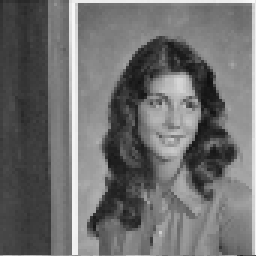
\includegraphics[width=5cm]{fotos/rostro/k2_1.png} }}%
    \qquad
    \subfloat[Metodo 2]{{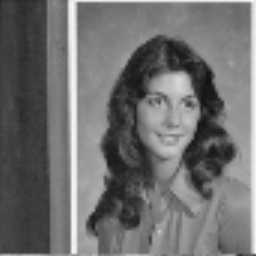
\includegraphics[width=5cm]{fotos/rostro/k2_2.png} }}%
    \qquad
    \subfloat[Metodo 3]{{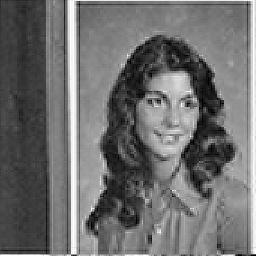
\includegraphics[width=5cm]{fotos/rostro/k2_3.png} }}%
    \caption{Comparacón de metodos para $k = 2$}%
    \label{fig:example}%
\end{figure}

Los artifact que vemos aquí son, bla bla bla (COMPLETAR!)
%metodo 1
%ECM        PSNR
%235.245    24.4156
%metodo 2
%87.1968    28.7258
%metodo 3
%295.885    23.4196
\\
Ahora lo hacemos para $k=3$, se obtiene esto:

\begin{figure}[H]
    \centering
    \subfloat[Metodo 1]{{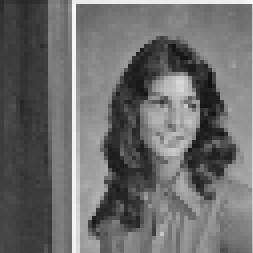
\includegraphics[width=5cm]{fotos/rostro/k3_1.png} }}%
    \qquad
    \subfloat[Metodo 2]{{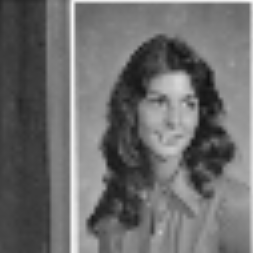
\includegraphics[width=5cm]{fotos/rostro/k3_2.png} }}%
    \qquad
    \subfloat[Metodo 3]{{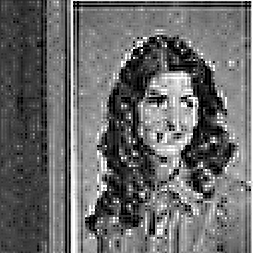
\includegraphics[width=5cm]{fotos/rostro/k3_3.png} }}%
    \caption{Comparacón de metodos para $k = 3$}%
    \label{fig:example}%
\end{figure}

%metodo 1
%ECM        PSNR
%389.559    22.2251
%metodo 2
%113.193    27.5926
%metodo 3
%1509.43    16.3427